\section{Mediciones}

\subsection{Construcción de las entradas}

Para generar los archivos de entrada hicimos un script en lenguaje Python.

El primer bloque de código genera un archivo llamado ``medicionesConSpanVariable.in''. Se fijan primero las constantes \emph{h}, \emph{carga}, \emph{C} y \emph{fMax}
(Las dos últimas no serán utilizadas, se agregan por consistencia, la carga se usará para todas las juntas por igual y será fija, al igual que la altura). 
Luego se procede a ciclar el span entre un valor mínimo y uno máximo, aumentando en 1 su valor, lo mismo se hace para \emph{n}, en un ciclo interno. 
Como resultado el archivo tendrá varias instancias separadas por líneas en blanco, con el mismo formato que pide la cátedra, con altura y cargas fijas, y span y secciones variables.

El segundo bloque de código hace algo muy parecido, generando el archivo llamado ``medicionesConCargaVariable.in''. En vez de fijar \emph{carga} se fijará \emph{span}, y se
procederá a ciclar entre cargas mínimas y máximas.
Éste archivo tendrá varias instancias separadas por líneas en blanco, con altura y span fijo, y cargas y secciones variables.


\subsection{Resultados}

\subsubsection{Span Variable}

\begin{figure}[H]
  \centering
    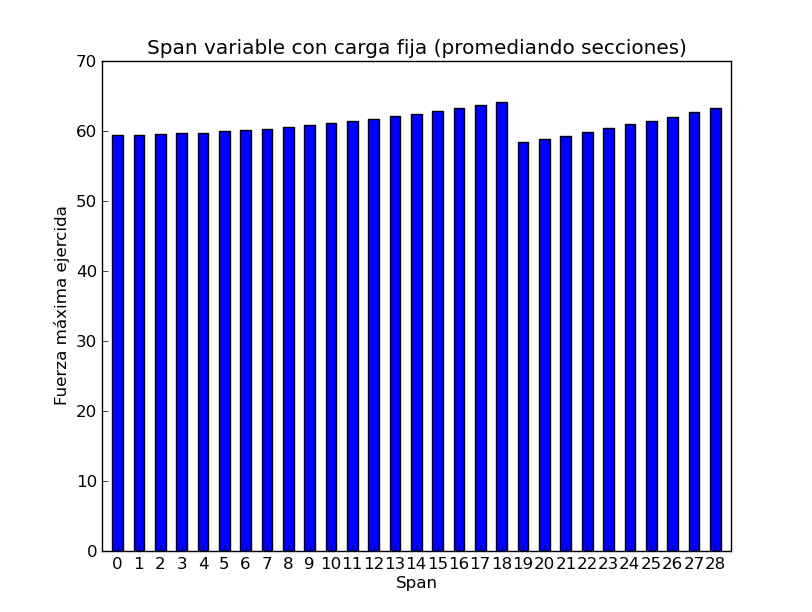
\includegraphics[width=0.9\textwidth]{../mediciones/spanVariable.png}
    \caption{}
\end{figure}



\subsubsection{Carga Variable}

\begin{figure}[H]
  \centering
    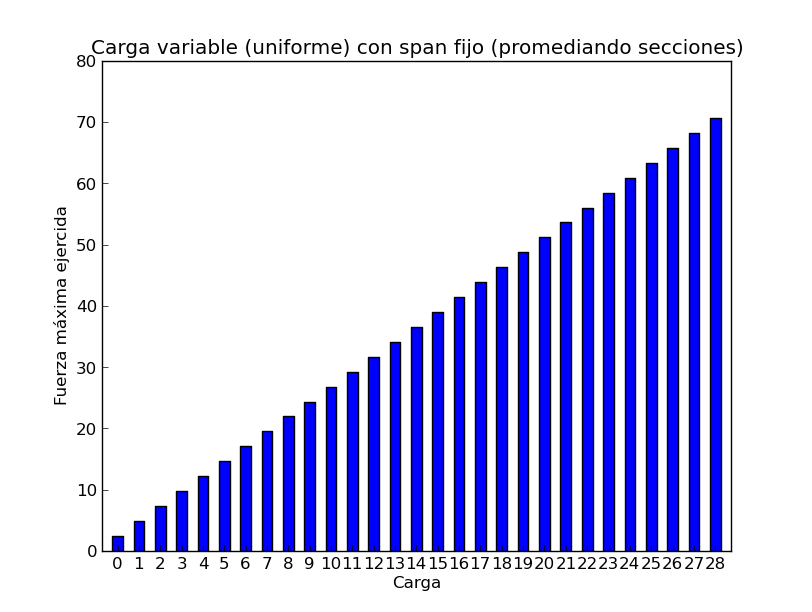
\includegraphics[width=0.9\textwidth]{../mediciones/cargaVariable.png}
    \caption{Error relativo final para distintos valores de tolerancia en el criterio de parada utilizando el cero de $x^2-\alpha$ con el método de Newton para cada orden de magnitud medido.}
\end{figure}